\section{Data and Analysis}
\label{sec:data}

In this section, we present the results of this study considering
each research question. 

\subsection{RQ1 Analysis}

RQ1 investigates whether the use of the recommender system can help
improve the effectiveness of test case prioritization techniques.
Figure~\ref{fig:All} shows the results combined for all applications.
The vertical axis shows APFD scores, and the horizontal axis shows 
prioritization techniques:
``$T_{ch}$'' (change impact-based), ``$T_{mfw}$'' (frequent web form-based), 
``$T_{mfm}$'' (frequent component-based), ``$T_{r}$'' (random order) and 
``$T_{hcf}$'' (recommender system-based). 

As shown in Figure~\ref{fig:All}, the proposed technique ($T_{hcf}$) 
yielded higher APFD scores than all control techniques while its data 
distribution is slightly wider than others. 
In particular, $T_{hcf}$ outperformed $T_{r}$ by 56\% in APFD 
score (the median APFD values for $T_{hcf}$ and $T_{r}$ are 80.59 and
59.39, respectively). 

The first three control techniques produced very similar results 
with marginal differences.
To understand how these techniques performed for each individual
application, we constructed boxplots for each application.
 
\begin{figure}[!ht]
%	\vspace*{-20pt}
	\centering
	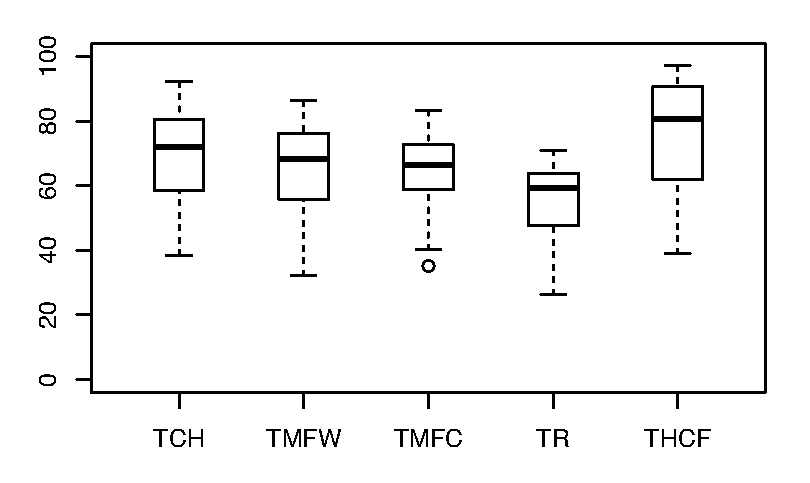
\includegraphics[width=1.05\linewidth]{./Total_adjusted.eps}
	\vspace*{-10pt}
	\caption{APFD Values for All Applications}
	\label{fig:All}
\end{figure} 

\begin{figure}[!ht]
	\centering
	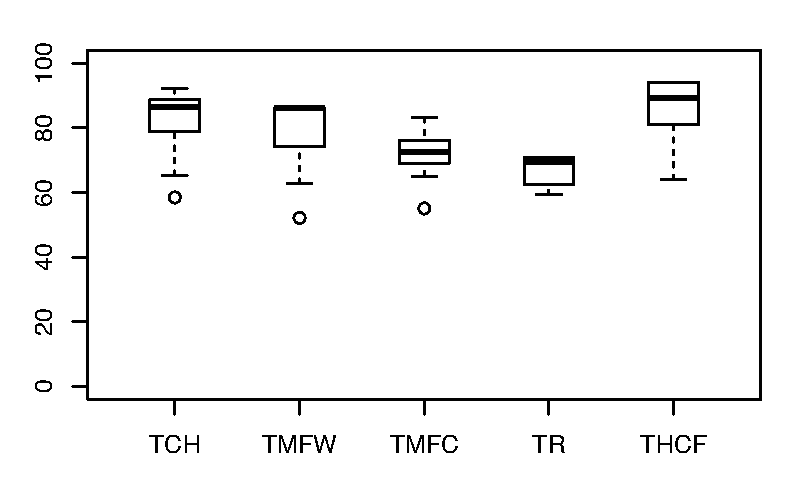
\includegraphics[width=1.05\linewidth]{./DASCP2_adjusted.eps}
	\vspace*{-10pt}
	\caption{DASCP - APFD Boxplots}
	\label{fig:DASCP}
\end{figure}

Figure ~\ref{fig:DASCP} presents the results for DASCP.
Similar to the results that considered all applications, 
the heuristic ($T_{hcf}$) outperformed all control techniques,
but data distribution patterns are different.  
The variances are small, but there are more outliers.
Among control techniques, the random technique was 
 the worst performer, whereas the frequent component-based technique ($T_{mfm}$)
produced results similar to the change history based technique ($T_{ch}$) .

Figure~\ref{fig:nopCommerce} presents the results for nopCommerce.
The results show that our proposed technique outperformed  
all four control techniques, but the variance of the APFD scores is relatively high. 
Among the first three control techniques, the change history-based 
technique ($T_{ch}$) produced slightly better results than the others.
This application has 23 versions, and we had a sufficient
amount of change history data for our training, so we speculate that
this is the reason why the change history-based technique produced 
better results than the two control techniques. 

\begin{figure}[!ht]
	\centering
	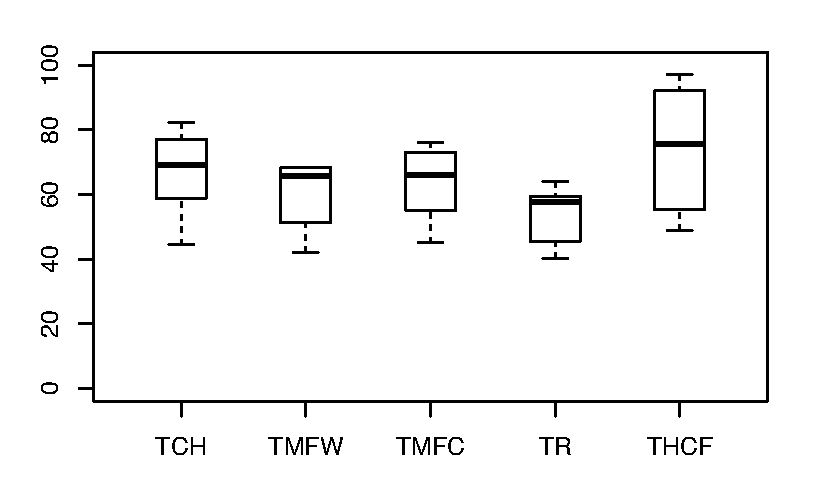
\includegraphics[width=1.05\linewidth]{./nop_adjusted.eps}
	\vspace*{-10pt}
	\caption{nopCommerce - APFD Boxplots}
	\label{fig:nopCommerce}
\end{figure}

Figure~\ref{fig:Coevery} shows the results for Coevery. 
When we compared the median values, our heuristic technique improved
the rate of fault detection by 21\% over the first three techniques 
on average and 41\% over the random technique. 
Among the first three control techniques, $T_{ch}$ and $T_{tmfw}$ 
produced slightly better results than $T_{mcf}$.

\begin{figure}[!ht]
	\centering
	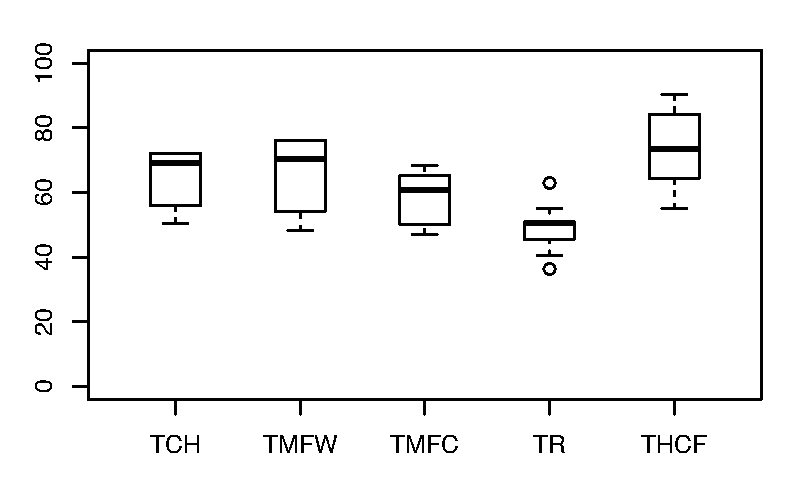
\includegraphics[width=1.05\linewidth]{./Coevery3_adjusted.eps}
	\vspace*{-10pt}
	\caption{Coevery - APFD Boxplots}
	\label{fig:Coevery}
\end{figure}

Overall, the experimental results showed that our proposed recommender 
system-based technique performed better than all the control techniques 
across all three applications. 
Among the control techniques, the random performed performed worst across all applications,
whereas the change history-based technique produced slightly better and more stable   
results for all applications.

\begin{table*}[!ht]
\caption{NAPFD Scores on Average.}
\vspace*{-10pt}
\begin{center}
\begin{tabular}{|c|c|c|c|c|c|c||c|c|c|c|}\hline
Application & Test Exe. & \multicolumn{5}{c||} {Techniques} 
& \multicolumn{4}{c|} {Improvement Rate over Control} \\\hline \hline
& Rate (\%)  & $T_{ch}$ & $T_{mfw}$ & $T_{mfm}$ & $T_{r}$ & $T_{hcf}$ 
& $T_{hcf}/T_{ch} $& $T_{hcf}/T_{mfw} $ & $T_{hcf}/T_{mfm}$ & $T_{hcf} /T_{r} $  \\\hline \hline
 
 &10	&18.54	&12.17	&15.12	&14.33	&23.37	&26\%	&92\%	&54\%	&63\%	\\
 &20	&21.31	&12.88	&16.78	&15.51	&29.98	&40\%	&132\%	&78\%	&93\%	\\
 &30	&28.86	&21.19	&25.12	&18.47	&40.95	&41\%	&93\%	&63\%	&121\%	\\
 &40	&40.42	&29.86	&38.68	&25.59	&55.3	&36\%	&85\%	&42\%	&116\%	\\
 DASCP &50	&54.34	&36.21	&42.9	&39.15	&67.07	&23\%	&85\%	&56\%	&71\%	\\
 &60	&61.7	&47.31	&50.34	&45.29	&70.42	&14\%	&48\%	&39\%	&55\%	\\
 &70	&68.34	&56.96	&65.97	&60.74	&76.67	&12\%	&34\%	&16\%	&26\%	\\
 &80	&75.41	&69.04	&71.14	&64.88	&84.01	&11\%	&21\%	&18\%	&29\%	\\
 &90	&83.35	&77.28	&77.69	&67.11	&89.83	&7\%	&16\%	&15\%	&33\%	\\
 &100	&90.16	&84.21	&79.22	&70.91	&94.14	&4\%	&11\%	&18\%	&32\%	\\\hline \hline
 
&10	&17.54	&12.17	&15.75	&8.33	&28.14	&60\%	&131\%	&78\%	&237\%	\\
&20	&29.28	&19.88	&28.35	&12.51	&47.9	&63\%	&140\%	&68\%	&282\%	\\
&30	&38.86	&27.19	&35.45	&15.57	&55.28	&42\%	&103\%	&55\%	&255\%	\\
&40	&44.42	&34.86	&48.68	&27.59	&65.06	&46\%	&86\%	&33\%	&135\%	\\
nopCommerce&50	&58.34	&39.16	&54.94	&35.91	&74.78	&28\%	&90\%	&36\%	&108\%	\\
&60	&62.7	&51.42	&57.08	&41.45	&81.49	&29\%	&58\%   &42\%	&96\%	\\
&70	&68.14	&55.03	&59.97	&50.02	&86.38	&26\%	&56\%   &44\%	&72\%	\\
&80	&76.22	&60.21	&64.14	&58.15	&89.87	&17\%	&49\%	&40\%	&54\%	\\
&90	&79.4	&66.01	&70.22	&60.17	&95.14	&19\%	&44\%	&35\%	&58\%	\\
&100	&82.16	&68.32	&76.04	&63.91	&97.06	&18\%	&42\%	&27\%	&51\%	\\\hline \hline

&10	&26.54	&23.17	&29.12	&20.33	&41.02	&54\%	&77\%	&40\%&	101\%	\\
&20	&44.28	&42.88	&45.12	&24.51	&66.98	&51\%	&56\%	&48\%	&173\%\\
&30	&60.86	&44.19	&50.12	&28.57	&73.28	&20\%	&65\%	&46\%	&156\%	\\
&40	&63.42	&51.51	&53.68	&31.59	&75.06	&18\%	&45\%	&39\%	&137\%	\\
Coevery &50	&64.34	&55.74	&58.3	&39.62	&77.1	&19\%	&38\% 	&32\%&	94\%	\\
&60	&66.7	&56.33	&60.41	&44.09	&78.65	&17\%	&39\% 	&30\%	&78\%\\
&70	&68.19	&59.86	&62.97	&46.11	&81.13	&18\%	&35\%	&28\%	&75\%	\\
&80	&70.67	&66.1	&65.14	&57.91	&83.2	&17\%	&25\%	&27\%	&43\%	\\
&90	&71.81	&73.14	&66.03	&59.01	&86.69	&20\%	&18\%	&31\%	&46\%	\\
&100	&72.16	&76.21	&68.22	&62.91	&87.23	&20\%	&14\% 	&27\%	&38\%	\\\hline 

\end{tabular}
\end {center}
\label{tab:napfd}
\vspace*{-5pt}
\end{table*}

\subsection{RQ2 Analysis}

RQ2 investigates whether the use of the recommender system can improve the effectiveness
of test prioritization when we have a limited budget for testing. 
In RQ2 analysis, we measured NAPFD, which is a normalized ratio of APFD, when 
our resources were not consistent.
In this experiment, first we executed 10\% of our test cases, and we continued to execute the
test cases in increments of 10\% of the total until they had all been  
executed to see whether we could improve the fault detection rate given a 
time constraint dictating that running 100\% of the test cases at one time was not feasible. 

Table~\ref{tab:napfd} shows the results of our three applications.
This table shows the results of two primary analyses. The first part of the table 
presents the NAPFD scores on average, and the second part shows the 
improvement rates of the heuristic technique over the four other control techniques. 

By examining the numbers in the table, we can observe that the improvement
rates of our heuristic technique over the control techniques vary widely. 
When we compared the heuristic with $T_{ch}$, the improvement rates ranged from
4\% to 41\% for DASCP, from 17\% to 63\% for nopCommerce, and from 17\% to 54\%
for Coevery.
When compared with $T_{mfw}$, the improvement rates ranged from
11\% to 132\% for DASCP, from 42\% to 140\% for nopCommerce, and from 14\% to 77\%
for Coevery, indicating significant improvements. 
When compared with $T_{mfm}$, the improvement rates ranged from
15\% to 78\% for DASCP, from 27\% to 78\% for nopCommerce, and from 27\% to 48\%
for Coevery, indicating results similar to those for as $T_{ch}$.
As for the comparison with $T_{r}$, the results were more remarkable.
The rates ranged from 32\% to 282\% for all three applications. 

One outstanding trend we observed in the table is that the improvement 
rates are much higher when the time budget is smaller.
For example, in the comparison with $T_{ch}$ for nopCommerce, 
when 10\% of budget was assigned, the improvement rate was 60\%,
but when we had a full budget, the rate dropped to 18\%.
A similar trend can be observed across all control techniques and applications.  
This indicates that our approach can be more helpful when companies are operating
under a tight budget.

To visualize our results, we illustrate them in lineplots as shown in
Figures~\ref{fig:DASCP-npfd}, \ref{fig:nop-npfd}, and \ref{fig:coevery-npfd}. 
Examining the lineplots for DASCP (Figure~\ref{fig:DASCP-npfd}), we observe 
that the growth in NAPFD values for $T_{chf}$ and $T_{ch}$ trended upward quickly while 
running the first 50\% of test cases, becoming nearly stable for the rest 
of the test cases. This means that more defects were detected at a relatively
early stage of test execution when we applied these two techniques. 

In the case of nopCommerce (Figure~\ref{fig:nop-npfd}), we can see 
that in the first 20\% test executions, NAPFD value produced by the heuristic approach 
($T_{chf}$) increased dramatically.  
Also, there is a remarkable difference between the NAPFD scores of 
the heuristic technique and all the other control techniques at every stage of
test execution. The most significant difference between scores 
occurred during the time that we were running between 
20\% and 30\% of the test cases. 

As for of Coevery (Figure~\ref{fig:coevery-npfd}),
similar to nopCommerce, it is evident that after 10\% of test case execution, 
the NAPFD value produced by the heuristic technique increased dramatically, but 
and after 20\% of test case execution 
the increase was not as significant, in fact becoming stable.

We can infer that a great number of defects can be 
detected at a very early stage of test case execution when applying our approach
to nopCommerce and Coevery, looking at the figures for those two applications.

\begin{figure}[!ht]
        \centering
        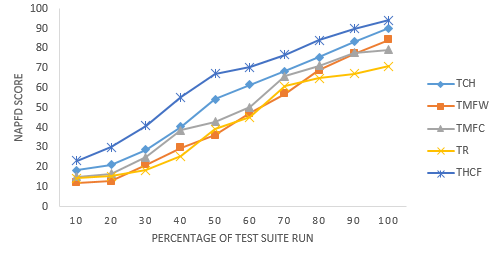
\includegraphics[width=1.0\linewidth]{./DASCP-npfd.png}
%       \vspace*{3pt}
        \caption{DASCP- NAPFD lineplots}
        \label{fig:DASCP-npfd}
\end{figure}

\begin{figure}[!ht]
        \centering
        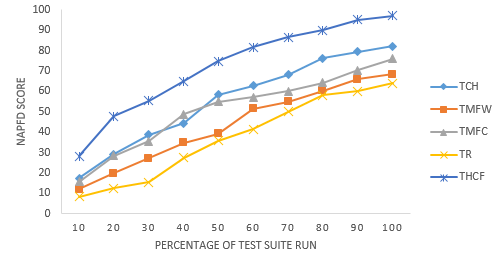
\includegraphics[width=1.0\linewidth]{./nop-npfd.png}
%       \vspace*{3pt}
        \caption{nopCommerce- NAPFD lineplots}
        \label{fig:nop-npfd}
\end{figure}

\begin{figure}[!ht]
        \centering
        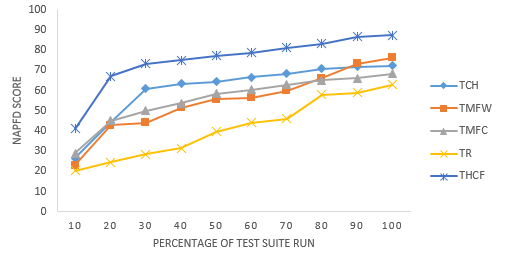
\includegraphics[width=1.0\linewidth]{./Coevery-npfd.png}
%       \vspace*{3pt}
        \caption{Coevery- NAPFD lineplots}
        \label{fig:coevery-npfd}
\end{figure}


